\documentclass[11pt,a4paper]{article}

\usepackage[margin=2.4cm]{geometry}
\usepackage[T1]{fontenc}
\usepackage{amsmath,amssymb}
\usepackage{array,booktabs}
\usepackage{xcolor}
\usepackage{tikz}
\usetikzlibrary{arrows.meta,positioning,shapes.geometric}
\usepackage[hidelinks]{hyperref}

\definecolor{accent}{HTML}{1E5AA8}
\definecolor{softblue}{HTML}{EAF2FB}
\hypersetup{
  colorlinks=true,
  linkcolor=accent,
  urlcolor=accent,
  citecolor=accent,
  pdftitle={Fixture LaTeX para teste do bp-viewer},
  pdfauthor={bp-viewer}
}

\title{Fixture LaTeX para teste do bp-viewer}
\author{Documento de validação manual}
\date{\today}

\begin{document}

\maketitle
\begin{abstract}
Este documento é um fixture deliberadamente pequeno, mas com vários elementos
que exercitam o preview PDF: índice, várias páginas, referências cruzadas,
matemática, tabela, listas, links, uma figura vetorial local incluída por
\verb|\input| e bibliografia. O texto também serve para testar seleção e cópia.
\end{abstract}

\tableofcontents
\newpage

\section{Como usar este documento}
\label{sec:como-usar}

O ficheiro principal é \texttt{main.tex}. Abra-o no bp-viewer e confirme que a
compilação termina, que o PDF ocupa uma escala legível e que o scroll mantém a
posição. Este parágrafo contém texto contínuo suficiente para testar seleção,
cópia e pesquisa. Procure, por exemplo, a expressão \emph{invariante de
preview}, que aparece também mais à frente.

Há uma dependência local simples, \texttt{fixture-diagram.tex}, usada na
Figura~\ref{fig:pipeline}. Alterar esse ficheiro deve invalidar o preview do
root. A referência interna \hyperref[sec:matematica]{para a secção de
matemática} deve navegar para a página correta, tal como o link de regresso ao
\hyperref[sec:como-usar]{início deste teste}.

\subsection{Checklist visual incorporada}
\label{subsec:checklist}
Esta lista torna fácil confirmar vários elementos no PDF:
\begin{itemize}
  \item títulos e índice clicável;
  \item texto selecionável e pesquisável;
  \item referência à equação~\eqref{eq:invariante};
  \item tabela com várias colunas;
  \item figura vetorial gerada localmente;
  \item link externo para \href{https://www.latex-project.org/}{latex-project.org}.
\end{itemize}

\paragraph{Nota de interação.}
O link externo deve abrir apenas quando clicado explicitamente. Os links
internos devem navegar dentro do PDF sem abrir ficheiros no Finder.

\newpage
\section{Modelo, equação e referências}
\label{sec:matematica}

Considere uma sequência de gerações de preview. Uma forma compacta de a
descrever é:
\begin{equation}
  P_{n+1} = \operatorname{publish}\!\left(\operatorname{render}(S_n,D_n,C)\right),
  \qquad n \in \mathbb{N},
  \label{eq:invariante}
\end{equation}
onde $S_n$ representa o snapshot de fontes, $D_n$ as dependências observadas e
$C$ a configuração do compilador. A equação~\eqref{eq:invariante} é uma
referência cruzada real; a página pode ser encontrada através de
\pageref{eq:invariante}.

A publicação deve aceitar apenas um artefacto válido. Em termos simples,
podemos escrever a condição de segurança como
\[
  \text{publicar}(p) \Longleftrightarrow
  \text{geração}(p)=\text{geração atual}\ \land\ p\text{ começa por }\texttt{\%PDF}.
\]
Este bloco testa símbolos matemáticos, texto monoespaçado e a renderização de
uma fórmula destacada.

\subsection{Tabela de cenários}
\label{subsec:tabela}

\begin{table}[ht]
  \centering
  \caption{Cenários manuais cobertos pelo fixture.}
  \label{tab:cenarios}
  \begin{tabular}{@{}>{\raggedright\arraybackslash}p{3.4cm}p{7.6cm}c@{}}
    \toprule
    Elemento & O que observar no bp-viewer & Prioridade \\
    \midrule
    Índice & Entradas clicáveis e hierarquia de secções & Alta \\
    Referências & \verb|\eqref|, \verb|\ref| e \verb|\pageref| & Alta \\
    Dependência & Alteração de \texttt{fixture-diagram.tex} & Alta \\
    Bibliografia & Citação e lista final após BibTeX & Média \\
    Links & Destino interno e URL externa explícita & Média \\
    \bottomrule
  \end{tabular}
\end{table}

Como mostra a Tabela~\ref{tab:cenarios}, a dependência local é um cenário de
prioridade alta. A citação de um livro clássico sobre tipografia digital
aparece aqui para exercitar a cadeia BibTeX~\cite{knuth1984texbook}.
Para manter a lista de referências suficientemente visível no teste, a
segunda entrada local também é incluída sem citação no corpo do texto.
\nocite{mittelbach2004latex}

\subsection{Texto para scroll e pesquisa}
\label{subsec:scroll}

O preview deve mostrar várias páginas contínuas e manter uma posição estável
quando o leitor percorre o documento. Este bloco repete frases intencionais
para tornar a pesquisa útil. A invariante de preview liga a geração, o
snapshot, as dependências e o PDF. A invariante de preview não deve mudar só
porque o leitor fez scroll. A invariante de preview deve continuar legível em
zoom reduzido e ampliado.

\begin{enumerate}
  \item Abra o índice e salte para a secção~\ref{sec:matematica}.
  \item Pesquise ``invariante de preview'' e percorra os resultados.
  \item Selecione este texto e copie-o com \texttt{Cmd+C}.
  \item Use o link \hyperref[sec:figura]{para a figura} e volte com o link
        \hyperref[sec:como-usar]{para o início}.
\end{enumerate}

\newpage
\section{Figura e dependência local}
\label{sec:figura}

A figura abaixo é produzida por TikZ a partir do ficheiro local
\texttt{fixture-diagram.tex}. Não exige conversores, shell escape ou imagens
binárias externas, por isso deve ser estável no TeX Live atualmente instalado.
\begin{figure}[ht]
  \centering
  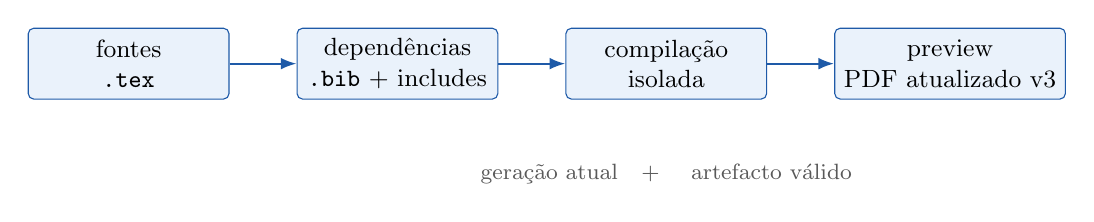
\begin{tikzpicture}[
  node distance=1.25cm and 0.85cm,
  box/.style={draw=accent, fill=softblue, rounded corners=2pt,
              minimum width=2.55cm, minimum height=0.9cm,
              align=center, font=\small},
  arrow/.style={-{Latex[length=2mm]}, thick, draw=accent}
]
  \node[box] (source) {fontes\\\texttt{.tex}};
  \node[box, right=of source] (deps) {dependências\\\texttt{.bib} + includes};
  \node[box, right=of deps] (build) {compilação\\isolada};
  \node[box, right=of build] (pdf) {preview\\PDF atualizado v3};
  \draw[arrow] (source) -- (deps);
  \draw[arrow] (deps) -- (build);
  \draw[arrow] (build) -- (pdf);
  \node[below=0.7cm of build, align=center, font=\footnotesize, text=black!65]
    {geração atual\quad + \quad artefacto válido};
\end{tikzpicture}

  \caption{Pipeline visual do fixture e do preview.}
  \label{fig:pipeline}
\end{figure}

Na Figura~\ref{fig:pipeline}, o fluxo passa de fontes para dependências, depois
para compilação e finalmente para PDF. A Figura~\ref{fig:pipeline} também é
útil para testar zoom, nitidez e seleção de texto à volta de conteúdo gráfico.

\subsection{Outro bloco de texto}
\label{subsec:mais-texto}
O documento inclui deliberadamente margens confortáveis e linhas de texto
normais, para que o PDF seja legível tanto em janela larga como estreita. Ao
redimensionar a janela, a escala inicial deve continuar sensata. Depois de
visitar esta página, force uma atualização e confirme se o leitor regressa à
página atual em vez de saltar desnecessariamente para o topo.

Uma pequena nota com caracteres acentuados — ação, índice, ficheiro, geração,
posição e atualização — verifica que a cópia e a pesquisa preservam Unicode de
forma razoável. Também há pontuação, números 12345 e identificadores como
\texttt{main.tex}, \texttt{references.bib} e \texttt{fixture-diagram.tex}.

\newpage
\section{Conclusões do teste}
\label{sec:conclusoes}

Este fixture não é uma tese e não pretende cobrir engines que não estão
instaladas. O objetivo é fornecer um documento previsível para a primeira
ronda manual do bp-viewer. Deve ser possível abrir o root, ver o índice,
navegar entre pelo menos quatro páginas, pesquisar texto, selecionar conteúdo,
seguir referências, observar a figura e confirmar a bibliografia.

Para validar a atualização de dependências, altere uma cor ou o texto em
\texttt{fixture-diagram.tex}, guarde e aguarde a nova compilação. Para validar
uma falha recuperável, introduza temporariamente um comando inválido em
\texttt{main.tex}, observe o diagnóstico, reverta a alteração e use
``Tentar novamente''.

O resultado esperado é um preview PDF válido, com a bibliografia abaixo e sem
ficheiros auxiliares escritos na pasta raw pelo bp-viewer.

\clearpage
\addcontentsline{toc}{section}{Referências}
\bibliographystyle{plain}
\bibliography{references}

\end{document}
